Para otorgar permisos de lectura o escritura a roles y usuarios es necesario contar con permisos de administrador y estar en la perspectiva avanzada. Estos permisos deben aplicarse en el nivel del modelo de datos, espacio de datos y conjunto de datos.

\subsection{Modelo de datos} 

Para conceder permisos a un rol o usuario en un modelo de datos, primero hay que acceder a la sección de “Modelo de datos” y seleccionar el modelo correspondiente. Luego, ir al apartado de “Acciones” y, en el menú desplegable, elegir la opción “Permisos”.

\begin{figure}[H]
    \centering
    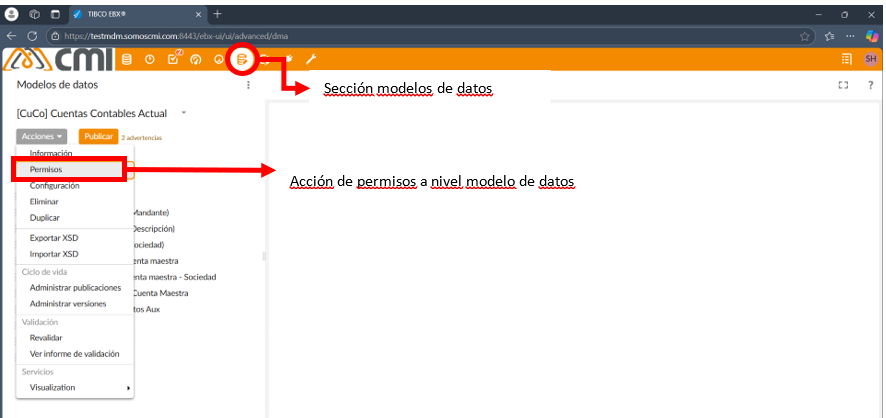
\includegraphics[width=0.8\textwidth]{RolesUsuario/ImgRolesUsuario/PRS01.png}
    \caption{Ubicación de Permisos dentro del modelo de datos.}
\end{figure}

Se despliega una ventana que muestra los roles y usuarios con permisos asignados en el modelo, junto con la opción de añadir nuevos permisos. Cada rol o usuario podrá realizar distintas funciones en cada sección como:

\begin{itemize}
    \item Lectura y escritura
    \item Solo lectura
    \item Ocultarlo
\end{itemize}

\begin{figure}[H]
    \centering
    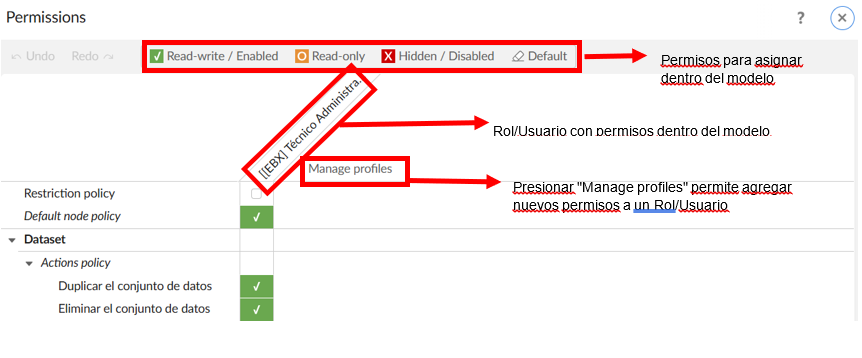
\includegraphics[width=0.8\textwidth]{RolesUsuario/ImgRolesUsuario/PRS02.png}
    \caption{Asignación de permisos en el modelo de datos}
\end{figure}

Cuando se marque el rol/usuario y tipo de permisos a asignar se debe “Guardar” para finalizar la asignación de permisos dentro un modelo.

\subsection{Espacio de datos}

Al ingresar a la sección de \textbf{“Espacio de Datos”}, se selecciona el espacio al que se desean otorgar permisos al rol o usuario. Dentro de este espacio, se accede al apartado “Acciones” y, posteriormente, se elige la opción “Permisos”.

\begin{figure}[H]
    \centering
    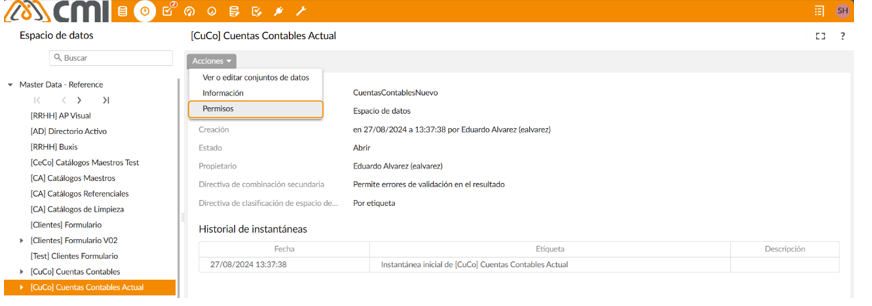
\includegraphics[width=0.8\textwidth]{RolesUsuario/ImgRolesUsuario/PRS03.png}
    \caption{Acción de Permisos en Espacio de Datos.}
\end{figure}

Se muestra una sección donde se pueden visualizar los roles y usuarios con permisos en el espacio de datos actual; además de la opción para agregar nuevos permisos.

\begin{figure}[H]
    \centering
    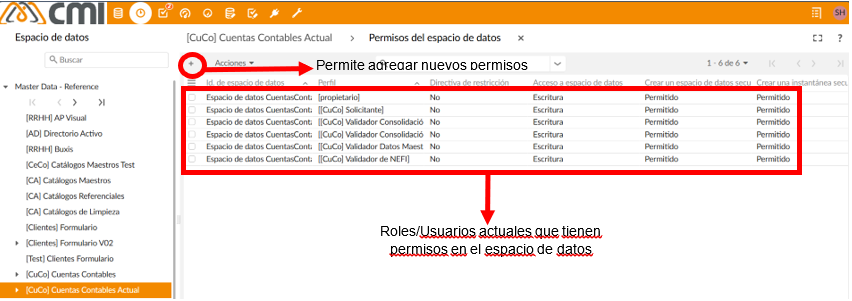
\includegraphics[width=0.8\textwidth]{RolesUsuario/ImgRolesUsuario/PRS04.png}
    \caption{Roles/Usuarios y sus permisos en el Espacio de Datos.}
\end{figure}

\subsection{Conjunto de Datos}


Al ingresar a la sección de datos, seleccionar el conjunto de datos al que se quiere otorgar permisos para el rol o usuario especifico. Dentro de este conjunto de datos, hay que dirigirse al apartado “Acciones” y, en el menú desplegable, elegir la opción “Permisos”.

\begin{figure}[H]
    \centering
    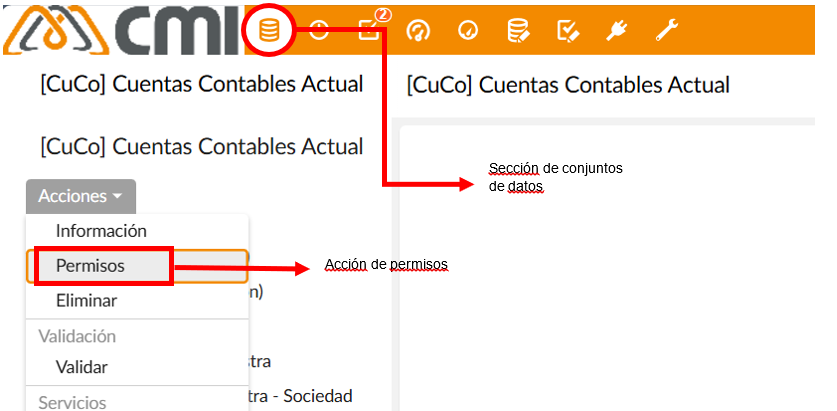
\includegraphics[width=0.8\textwidth]{RolesUsuario/ImgRolesUsuario/PRS05.png}
    \caption{Acción de Permisos en el Conjunto de Datos.}
\end{figure}

Se despliega una ventana que muestra los roles y usuarios con permisos asignados en el modelo, junto con la opción de añadir nuevos permisos. Cada rol o usuario podrá realizar distintas funciones en cada sección como:

\begin{itemize}
    \item Lectura y escritura
    \item Solo lectura
    \item Ocultarlo
\end{itemize}

\begin{figure}[H]
    \centering
    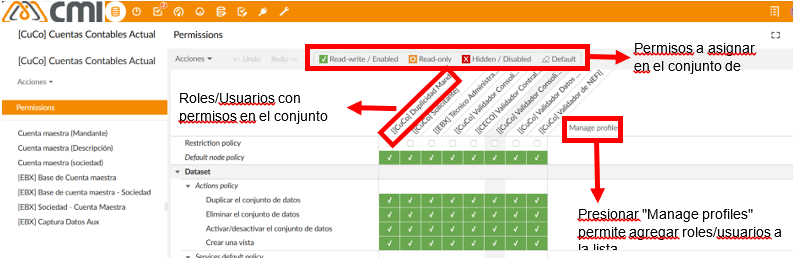
\includegraphics[width=0.8\textwidth]{RolesUsuario/ImgRolesUsuario/PRS06.png}
    \caption{Permisos asignados dentro del conjunto de datos.}
\end{figure}

Cuando se marque el rol/usuario y tipo de permisos a asignar se debe \textbf{“Guardar”} para finalizar la asignación de permisos dentro del conjunto de datos.



